% %% %%%%%%%%%%%%%%%%%%%%%%%%%%%%%%%%%%%%%%%%%%%%%%%%%%%%%%%%%%
% intro-lm35.tex
%
% Author:  Mauricio Matamoros
% License: MIT
%
% %% %%%%%%%%%%%%%%%%%%%%%%%%%%%%%%%%%%%%%%%%%%%%%%%%%%%%%%%%%%

%!TEX root = ../practica.tex
%!TEX root = ../references.bib

\subsection{El sensor LM35}%
\label{sec:intro-lm35}
El circuito integrado LM35 es un sensor de temperatura cuya salida de voltaje o respuesta es linealmente proporcional a la temperatura registrada en escala centígrada.
Una de las principales ventajas del LM35 sobre otros sensores lineales calibrados en Kelvin, es que no se requiere restar constantes grandes para obtener la temperatura en grados centígrados.
El rango de este sensor va de \degreesC{-55} a \degreesC{150} con una precisión que varía entre \degreesC{0.5} y \degreesC{1.0} dependiendo la temperatura medida~\Citep{LM35datasheet}.

\begin{figure}
	\centering
	\begin{subfigure}[b]{0.5\columnwidth}
		\centering
		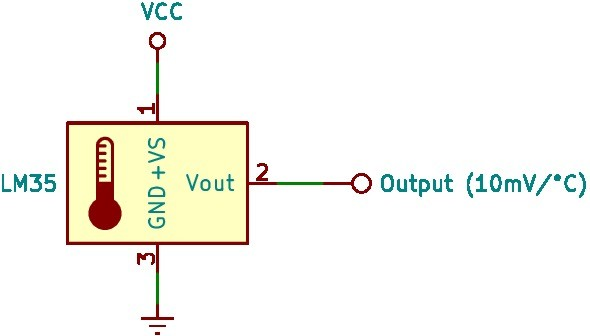
\includegraphics[width=\textwidth,height=5cm,keepaspectratio]{img/lm35a.jpg}
		\caption{Configuración básica: \degreesC{2} a \degreesC{150}}
		\label{fig:lm35config-a} %chktex 24
	\end{subfigure}%
	\begin{subfigure}[b]{0.5\columnwidth}
		\centering
		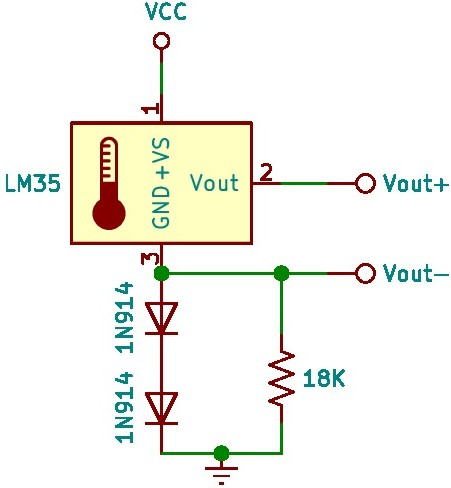
\includegraphics[width=\textwidth,height=5cm,keepaspectratio]{img/lm35b.jpg}
		\caption{Configuración clásica: \degreesC{-55} a \degreesC{150}}
		\label{fig:lm35config-b} %chktex 24
	\end{subfigure}
	\caption{Configuraciones típicas del LM35}
	\label{fig:lm35config} % chktex 24
\end{figure}

Las configuraciones más comunes para este integrado se muestran en la \Cref{fig:lm35config}. La configuración (\Cref{fig:lm35config-a}) básica, la más simple posible pues sólo requiere conectar al integrado LM35 entre \VCC y \GND, permite medir temperaturas entre \degreesC{2} a \degreesC{150}.
Por otro lado, la configuración (\Cref{fig:lm35config-a}) clásica permite medir en todo el rango completo del sensor, es decir entre \degreesC{-55} y \degreesC{150}, pero requiere de un par de diodos 1N914 y una resistencia de 18K$\Omega$ para proporcionar los voltajes de referencia.
En ambos casos, el LM35 ofrece una diferencial de $10mV/^{o}C$, por lo que los voltajes medidos rara vez excederán de 2V respecto a tierra.

Cuando opera en rango completo y las temperaturas registradas son inferiores a cero, se permite un flujo de corriente inverso entre los pines GND y V\textsubscript{out} del LM35, es decir, una salida de voltaje negativo respecto a la referencia.
Debido a que el LM35 no puede generar voltajes inferiores respecto a la referencia del circuito (tierra) se utilizan dos diodos 1N914 en serie colocados en el pin de referencia o tierra del LM35 (véase \Cref{fig:lm35config-b}) para elevar el voltaje del subcircuito del LM35 aproximadamente 1.2V por encima del voltaje de referencia o tierra general.
Así, cuando el LM35 entre en contacto con temperaturas negativas, el voltaje de diodo o V\textsubscript{DD} referenciable mediante la resistencia de 18K hará posible que el voltaje de V\textsubscript{out+} sea inferior al de V\textsubscript{out-} y pueda calcularse la diferencia, tal como se muestra en la~\Cref{tab:lm35}.

\begin{wraptable}{r}{7.0cm}
	\centering
	\caption{Salida de un LM35 en rango completo}%
	\label{tab:lm35} %chktex 24
	\begin{tabular}{rr}%\\
	\toprule
	Temp [\degreesC{}]& V\textsubscript{out+} [V] \\
	\midrule
	-55 & 0.65 \\
	  0 & 1.20 \\
	 50 & 1.70 \\
	100 & 2.20 \\
	150 & 2.70 \\
	\bottomrule
	\end{tabular}
\end{wraptable}
